
\chapter{Introduction to GUI programming}

Python has no native support for GUI (Graphical User Interface) programming, but this isn't a problem since many GUI libraries written in other languages can be used by Python programmers.
This is possible becuase many GUI libraries have Python \keyword{wrappers} or \keyword{bindings} -- these are packages and modules that are imported and used like any other Python packages and modules but which access functionality that is in non-Python libraries under the hood.


Python's standard library includes Tcl/Tk -- Tcl is an almost syntax-free scripting language and Tk is a GUI library written in Tcl and C.
Python's \verb|tkinker| module provides Python binding for the Tk GUI library.
Tk has three advantages compared with other GUI libraries:
\begin{itemize}
\item It is installed as standard with Python, so it is always available.
\item It is small.
\item It comes with IDLE.
\end{itemize}



For developing GUI programs that must run on any or all Python desktop platform, using only a standard Python installation with no additional libraries, there is just one choice: Tk.



\section{Dialog-style programs}

In most object-oriented programs, a custom class is used to represent a single main window or dialog, with most of the widgets it contains being instances of standard widgets, such as buttons or checkboxes, supplied by the library.
Like most cross-platform GUI libraries, Tk doesn't really make distinction between a window and a widget -- a window is simply a widget that has no widget parent.
Widgets that don't have a widget parent (windows) are automatically supplied with a frame and window decorations (such as a title bar and close button).
In addition to distinguishing between widgets and windows (also called top-level widgets), the parent–child relationships help ensure that widgets are deleted in the right order and that child widgets are automatically deleted when their parent is deleted.

The interface is shown in Figure \ref{fig:interest}.
\begin{figure}[!ht]
  \centering
  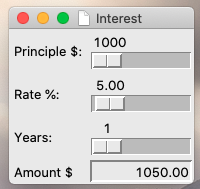
\includegraphics[width=0.8\textwidth]{pics/interest}
  \caption{The interest program}
  \label{fig:interest}
\end{figure}

The corresponding code is shown below:


\begin{lstlisting}
#!/usr/bin/env python3
"""
@project: python3
@file: interest
@author: mike
@time: 2021/2/23
 
@function:
"""
import tkinter
import os
import sys


class MainWindow(tkinter.Frame):
    def __init__(self, parent):
        super().__init__(parent)
        self.parent = parent
        # Lays out the frame using the grid layout manager
        self.grid(row=0, column=0)

        self.principal = tkinter.DoubleVar()
        self.principal.set(1000.0)
        self.rate = tkinter.DoubleVar()
        self.rate.set(5.0)
        self.years = tkinter.IntVar()
        self.amount = tkinter.StringVar()

        principal_label = tkinter.Label(self, text='Principle $:',
                                        anchor=tkinter.W,
                                        underline=0)
        principal_scale = tkinter.Scale(self, variable=self.principal,
                                        command=self.updateUi,
                                        from_=100,
                                        to=10000000,
                                        resolution=100,
                                        orient=tkinter.HORIZONTAL)
        rate_label = tkinter.Label(self, text='Rate %:',
                                   underline=0,
                                   anchor=tkinter.W)
        rate_scale = tkinter.Scale(self, variable=self.rate,
                                   command=self.updateUi,
                                   from_=1,
                                   to=100,
                                   resolution=0.25,
                                   digits=5,
                                   orient=tkinter.HORIZONTAL)
        year_label = tkinter.Label(self, text='Years:',
                                   underline=0,
                                   anchor=tkinter.W)
        year_scale = tkinter.Scale(self, variable=self.years,
                                   command=self.updateUi,
                                   from_=1,
                                   to=50,
                                   orient=tkinter.HORIZONTAL)
        amount_label = tkinter.Label(self, text='Amount $', anchor=tkinter.W)
        actual_amount_label = tkinter.Label(self, textvariable=self.amount,
                                            relief=tkinter.SUNKEN,
                                            anchor=tkinter.E)

        principal_label.grid(row=0, column=0, padx=2, pady=2, sticky=tkinter.W)
        principal_scale.grid(row=0, column=1, padx=2, pady=2, sticky=tkinter.EW)
        rate_label.grid(row=1, column=0, padx=2, pady=2, sticky=tkinter.W)
        rate_scale.grid(row=1, column=1, padx=2, pady=2, sticky=tkinter.EW)
        year_label.grid(row=2, column=0, padx=2, pady=2, sticky=tkinter.W)
        year_scale.grid(row=2, column=1, padx=2, pady=2, sticky=tkinter.EW)
        amount_label.grid(row=3, column=0, padx=2, pady=2, sticky=tkinter.W)
        actual_amount_label.grid(row=3, column=1, padx=2, pady=2, sticky=tkinter.EW)

        principal_scale.focus_set()
        self.updateUi()
        parent.bind('<Alt-p>', lambda *ignore: principal_scale.focus_set())
        parent.bind('<Alt-r>', lambda *ignore: rate_scale.focus_set())
        parent.bind('<Alt-y>', lambda *ignore: year_scale.focus_set())
        parent.bind('<Control-q>', self.quit)
        parent.bind('<Escape>', self.quit)

    def updateUi(self, *ignore):
        amount = self.principal.get() * (
                (1 + (self.rate.get() / 100.0)) ** self.years.get()
        )
        self.amount.set(f'{amount:.2f}')

    def quit(self, event=None):
        self.parent.destroy()


application = tkinter.Tk()
path = os.path.join(os.path.dirname(__file__), 'images/')
if sys.platform.startswith('win'):
    icon = path + 'interest.ico'
else:
    icon = '@' + path + 'interest.xbm'
application.iconbitmap(icon)
application.title('Interest')
window = MainWindow(application)
application.protocol('WM_DELETE_WINDOW', window.quit)
application.mainloop()
  
\end{lstlisting}




Rather than using absolute positions and sizes, widgets are laid out inside other widgets using layout managers.
The call to \verb|grid()| lays out the frame using the grid layout manager.
Every widget that is shown must be laid out, even top-level ones.


(Line 22-27)
Tk allows us to create variables that are associated with widgets.
If a variable’s value is changed programmatically, the change is reflected in its associated widget, and similarly, if the user changes the value in the widget the associated variable’s value is changed.


(Line 29-59)
This part of the initializer is where we create the widgets.
The \verb|tkinter.Label| widget is used to display read-only text to the user.
Like all widgets it is created with a parent, and then keyword arguments are used to set various other aspects of the widget’s behavior and appearance.
We have set the \verb|principalLabel|’s text appropriately, and set its anchor to \verb|tkinter.W|, which means that the label’s text is aligned west (left).
The underline parameter is used to specify which character in the label should be underlined to indicate a keyboard accelerator (e.g., Alt+P).
(A keyboard accelerator is a key sequence of the form \verb|Alt+letter| where \verb|letter| is an underlined letter and which results in the keyboard focus being switched to the widget associated with the accelerator, most commonly the widget to the right or below the label that has the accelerator.)


(Line 72-77)
We set up a few key bindings.


To give the program an icon on Windows we use an \keyword{.ico} file and pass the name of the file (with its full path) to the iconbitmap() method.
But for Unix platforms we must provide a bitmap.
Tk has several built-in bitmaps, so to distinguish one that comes from the file system we must precede its name with an \keyword{@} symbol.



\section{Main-window-style programs}

\url{https://github.com/mikechyson/python3/blob/master/c15_gui/bookmarks_tk.pyw}